\documentclass[english,man]{apa6}

\usepackage{amssymb,amsmath}
\usepackage{ifxetex,ifluatex}
\usepackage{fixltx2e} % provides \textsubscript
\ifnum 0\ifxetex 1\fi\ifluatex 1\fi=0 % if pdftex
  \usepackage[T1]{fontenc}
  \usepackage[utf8]{inputenc}
\else % if luatex or xelatex
  \ifxetex
    \usepackage{mathspec}
    \usepackage{xltxtra,xunicode}
  \else
    \usepackage{fontspec}
  \fi
  \defaultfontfeatures{Mapping=tex-text,Scale=MatchLowercase}
  \newcommand{\euro}{€}
\fi
% use upquote if available, for straight quotes in verbatim environments
\IfFileExists{upquote.sty}{\usepackage{upquote}}{}
% use microtype if available
\IfFileExists{microtype.sty}{\usepackage{microtype}}{}

% Table formatting
\usepackage{longtable, booktabs}
\usepackage{lscape}
% \usepackage[counterclockwise]{rotating}   % Landscape page setup for large tables
\usepackage{multirow}		% Table styling
\usepackage{tabularx}		% Control Column width
\usepackage[flushleft]{threeparttable}	% Allows for three part tables with a specified notes section
\usepackage{threeparttablex}            % Lets threeparttable work with longtable

% Create new environments so endfloat can handle them
% \newenvironment{ltable}
%   {\begin{landscape}\begin{center}\begin{threeparttable}}
%   {\end{threeparttable}\end{center}\end{landscape}}

\newenvironment{lltable}
  {\begin{landscape}\begin{center}\begin{ThreePartTable}}
  {\end{ThreePartTable}\end{center}\end{landscape}}

  \usepackage{ifthen} % Only add declarations when endfloat package is loaded
  \ifthenelse{\equal{\string man}{\string man}}{%
   \DeclareDelayedFloatFlavor{ThreePartTable}{table} % Make endfloat play with longtable
   % \DeclareDelayedFloatFlavor{ltable}{table} % Make endfloat play with lscape
   \DeclareDelayedFloatFlavor{lltable}{table} % Make endfloat play with lscape & longtable
  }{}%



% The following enables adjusting longtable caption width to table width
% Solution found at http://golatex.de/longtable-mit-caption-so-breit-wie-die-tabelle-t15767.html
\makeatletter
\newcommand\LastLTentrywidth{1em}
\newlength\longtablewidth
\setlength{\longtablewidth}{1in}
\newcommand\getlongtablewidth{%
 \begingroup
  \ifcsname LT@\roman{LT@tables}\endcsname
  \global\longtablewidth=0pt
  \renewcommand\LT@entry[2]{\global\advance\longtablewidth by ##2\relax\gdef\LastLTentrywidth{##2}}%
  \@nameuse{LT@\roman{LT@tables}}%
  \fi
\endgroup}


  \usepackage{graphicx}
  \makeatletter
  \def\maxwidth{\ifdim\Gin@nat@width>\linewidth\linewidth\else\Gin@nat@width\fi}
  \def\maxheight{\ifdim\Gin@nat@height>\textheight\textheight\else\Gin@nat@height\fi}
  \makeatother
  % Scale images if necessary, so that they will not overflow the page
  % margins by default, and it is still possible to overwrite the defaults
  % using explicit options in \includegraphics[width, height, ...]{}
  \setkeys{Gin}{width=\maxwidth,height=\maxheight,keepaspectratio}
\ifxetex
  \usepackage[setpagesize=false, % page size defined by xetex
              unicode=false, % unicode breaks when used with xetex
              xetex]{hyperref}
\else
  \usepackage[unicode=true]{hyperref}
\fi
\hypersetup{breaklinks=true,
            pdfauthor={},
            pdftitle={Equivalence Testing for Psychological Science},
            colorlinks=true,
            citecolor=blue,
            urlcolor=blue,
            linkcolor=black,
            pdfborder={0 0 0}}
\urlstyle{same}  % don't use monospace font for urls

\setlength{\parindent}{0pt}
%\setlength{\parskip}{0pt plus 0pt minus 0pt}

\setlength{\emergencystretch}{3em}  % prevent overfull lines

\ifxetex
  \usepackage{polyglossia}
  \setmainlanguage{}
\else
  \usepackage[english]{babel}
\fi

% Manuscript styling
\captionsetup{font=singlespacing,justification=justified}
\usepackage{csquotes}
\usepackage{upgreek}

 % Line numbering
  \usepackage{lineno}
  \linenumbers


\usepackage{tikz} % Variable definition to generate author note

% fix for \tightlist problem in pandoc 1.14
\providecommand{\tightlist}{%
  \setlength{\itemsep}{0pt}\setlength{\parskip}{0pt}}

% Essential manuscript parts
  \title{Equivalence Testing for Psychological Science}

  \shorttitle{Equivalence Testing}


  \author{Daniel Lakens\textsuperscript{1}, Anne M. Scheel\textsuperscript{1}, \& Peder Isager\textsuperscript{1}}

  \def\affdep{{"", "", ""}}%
  \def\affcity{{"", "", ""}}%

  \affiliation{
    \vspace{0.5cm}
          \textsuperscript{1} Eindhoven University of Technology  }

  \authornote{
    \newcounter{author}
    We would like to thank Courtney Soderbergh for creating the first
    version of the TOST function to test two independent proportions.

                      Correspondence concerning this article should be addressed to Daniel Lakens, Den Dolech 1, IPO 1.33, 5600 MB, Eindhoven, The Netherlands. E-mail: \href{mailto:D.Lakens@tue.nl}{\nolinkurl{D.Lakens@tue.nl}}
                                    }


  \abstract{Psychologists need to be able to test for the absence of an effect.
Using the Two-One-Sided Tests (TOST) procedure, researchers can easily
test whether the observed effects are too small to be meaningful. By
specifying a smallest effect size of interest (SESOI) researchers test
whether observed effects are surprisingly closer to zero, assuming there
was an effect the consider meaningful. We explain a range of approaches
to determine the SESOI in psychological science, and provide detailed
examples of how equivalence tests should be performed and reported.}
  \keywords{Equivalence Testing, NHST, power, TOST \\

    \indent Word count: X
  }





\usepackage{amsthm}
\newtheorem{theorem}{Theorem}
\newtheorem{lemma}{Lemma}
\theoremstyle{definition}
\newtheorem{definition}{Definition}
\newtheorem{corollary}{Corollary}
\newtheorem{proposition}{Proposition}
\theoremstyle{definition}
\newtheorem{example}{Example}
\theoremstyle{definition}
\newtheorem{exercise}{Exercise}
\theoremstyle{remark}
\newtheorem*{remark}{Remark}
\newtheorem*{solution}{Solution}
\begin{document}

\maketitle

\setcounter{secnumdepth}{0}



Psychologists should be able to falsify predictions. A common prediction
in psychological research is that an effect exists in the population
that differs from zero. For example, we might predict that priming
American Asian women with their Asian identify will increase their
performence on a math test compared to women in the control condition
who are primed with their female identity. To be able to falsify this
hypothesies, and design a study that allows for strong inferences
({\textbf{???}}), it is important to specify which test result would
\emph{disprove} the hypothesis.

An equivalence test can be used to test whether the observed effect is
surprisingly close to zero, assuming a meaningful effect exists in the
population. The test is a simple variation on the widely used null
hypothesis significance tests, with the small difference that instead of
testing the observed effect against zero, it is tested against a
smallest effect size of interest (SESOI). For example, if a difference
on a math test of 5\% or more is considered meaningful, one could test
against a SESOI of 5\%. If the observed effect is suprisingly closer to
0, assuming a true effect of 5\% or larger existed, one can declare
statistical equivalence, or reject the presence of effects that are
large enough to be considered meaningful. An equivalence test can be
used to falsify hypotheses.

One can conclude statistical equivalence whenever a 90\% confidence
interval around the effect size estimate does not contain the SESOI, or
when two one-sided tests (i.e., examining whether the difference on the
math test is more than -5\%, but less than 5\%) are statistically
significant. By combining null-hypothesis tests and equivalence tests,
four combinations of results can be observed (see Figure 1). Two
outcomes are straightforward to interpret, namely when the effect is
equivalent to zero, and not different from zero (an effect that is not
meaningful), and when the effect is not equivalent, and different from
zero (a meaningful effect). In addition, the effect can be different
from zero and too small to be considered meaningful (an effect which is
not meaningful) or the effect can neither differ from zero, not be
equivalent to zero (an undetermined result, where more data is needed).

Even though equivalence tests are just a small variation of traditional
Frequentist tests (testing against the SESOI, instead of 0), their use
was limited until the availability of user-friendly software to perform
the calculations (Lakens, 2017). In this article, we discuss different
approaches to determining the SESOI for psychological research, and
provide detailed reproducible examples of how to perform power analyses
when designing equivalence tests, and statistical re-analyses of
published psychology experiments.

\section{Justifying the Smallest Effect Size of
Interest}\label{justifying-the-smallest-effect-size-of-interest}

Equivalence tests are performed against a value that is considered the
smallest effect size of interest (SESOI). The SESOI can sometimes based
on just noticeable differences, which can be objectively determined.
Most often, however, it is a subjective decision that varies across
individuals and time. Both these approaches are valid, and even when a
just noticeable difference can be objectively determined, researchers
might choose to set the SESOI to a larger value. In many research areas,
the SESOI is best based on a cost-benefit analysis. Since both costs and
benefits are necessarily relative, the SESOI will depend on the
researcher who designs the study. The goal of setting a SESOI is to
clearly justify why designing a study that has a high probability of
rejecting effects larger than a specified value contributes to our
knowledge base. Researchers should not aim to determine a SESOI that is
universally valid. The goal is to set a SESOI such that inferences based
on it answer a meaningful question.

\subsection{Objective Justifications of a
SESOI}\label{objective-justifications-of-a-sesoi}

An objectively determined SESOI should be based on quantifiable
theoretical predictions, such as computational models. Sometimes, the
only theoretical prediction is that an effect should be noticeable. In
such circumstances, the SESOI can be set based on just noticeable
differences. For example, Burriss and colleagues ({\textbf{???}})
examined whether women displayed an increase in redness in the face
during the fertile phase of their ovulatory cycle. The hypothesis was
that a slighly redder skin signals greater attractiveness and physical
health, and sending this signal to men yields an evolutionary advantage.
This hypothesis requires that the increase in redness can be detected
with the naked eye by men. They collected data from 22 women and showed
that there was indeed an increase in redness of the facial skin of woman
during their fertile period. However, this increase was not large enough
to be noticeable with the naken eye by men, thus falsifying their
hypothesis. Because the just noticeable difference in redness of the
skin can be measured, it is possible to objectively establish the SESOI.

Another example of an objectively determined SESOI can be found in
({\textbf{???}}) where the minimal clinically important difference on
the Beck Depression Inventory - II was determined by asking 1039
patients when they subjectively felt less depressed (i.e., when they
personally noticed an improvement) and relating this to the
corresponding difference score on the depression inventory.

\subsection{Subjective justifications of a
SESOI}\label{subjective-justifications-of-a-sesoi}

We distinguish between three categories of subjective justifications for
SESOI. First, researchers can use benchmarks. For example, one might set
the SESOI to a standardized effect size of d = 0.5, which would allow
one to reject effect as large or larger than a \enquote{medium} effect
size (Cohen, 1988). Similarly, effect sizes smaller than a Cohen's d of
0.1 are sometimes considered trivially small (Maxwell, Lau, \& Howard,
2015). Relying on a benchmark is the weakest possible justification of a
SESOI, and should be avoided.

Second, researchers can determine the SESOI based on the literature.
Ideally, researchers would specify the SESOI in their research, but this
is not yet common practice. It is thus up to researchers who build on
earlier work to decide which effect size is too small to be meaningful,
given an earlier study. Simonsohn (2015) recently proposed to set the
SESOI to 33\% of the effect size an earlier study could detect based on
the sample size. For example, consider a study where 100 participants
answered a question, which was analyzed with an one-sample t-test. For a
two-sided test with an alpha of .05 this test had 33\% power to detect a
d = 0.15.

Another justifiable choice we would like to propose here is to use the
smallest observed effect size that could have been statistically
significant in the original study as the SESOI in a replication study.
Based only on the alpha level and the sample size, we can calculate the
criticial test value (e.g., \emph{t}, \emph{F}, \emph{Z}). This critical
test value can also be transformed to a standardized effect size (e.g.,
\(d = t \sqrt { \frac { 1} { n _ { 1} } + \frac { 1} { n _ { 2} } }\)),
which can thus be interpreted as a \emph{critical effect size}. All
observed effect sizes smaller than the critical effect size would not be
statistically significant in an original study, given the alpha and
sample size. By setting the SESOI to the critical effect size, an
equivalence test can reject all observed effect sizes that could have
been detected in an earlier study.

Third, researchers can set the SESOI based on the resources they have
available. The amount of data you can collect limits the inferences you
can make. Given a an alpha level and a sample size, researchers can
calculate the smallest effect size that can be rejected with the desired
power in an equivalence test. For example, a researcher who plans to
perform a two-sided one-sample t-test using an alpha of 5\%, based on
data from 100 observations, has 90\% power declare equivalence when
testing a SESOI of d = 0.33. Whether or not a test against a SESOI based
on the available resources contributes to the scientific literature
depends. One should not expect a test based on 11 observations, which
provides 90\% power to reject effects larger than d = 1, is particularly
informative, given that most effects in psychology are substantially
smaller than d = 1. But by transparently reporting the effects one can
detect and reject, based on the study design, researchers can
communicate the information their study contributes.

\[t _ { L } = \frac { M _ { 1} - M _ { 2} - \Delta _ { L } } { \sigma \sqrt { \frac { 1} { n _ { 1} } + \frac { 1} { n _ { 2} } } }, t _ { U } = \frac { M _ { 1} - M _ { 2} - \Delta _ { U } } { \sigma \sqrt { \frac { 1} { n _ { 1} } + \frac { 1} { n _ { 2} } } }
\]

\subsection{Examples}\label{examples}

\section{Equivalence test for
Meta-analysis}\label{equivalence-test-for-meta-analysis}

Hyde, Lindberg, Linn, Ellis, and Williams (2008) report that effect
sizes for gender differences in mathematics tests across the 7 million
students in the US represent trivial differences, where a trivial
difference is specified as an effect size smaller then d = 0.1. The
present a table with Cohen's d and se is reproduced below:

\begin{longtable}[]{@{}ll@{}}
\toprule
Grades & d + se\tabularnewline
\midrule
\endhead
Grade 2 & 0.06 +/- 0.003\tabularnewline
Grade 3 & 0.04 +/- 0.002\tabularnewline
Grade 4 & -0.01 +/- 0.002\tabularnewline
Grade 5 & -0.01 +/- 0.002\tabularnewline
Grade 6 & -0.01 +/- 0.002\tabularnewline
Grade 7 & -0.02 +/- 0.002\tabularnewline
Grade 8 & -0.02 +/- 0.002\tabularnewline
Grade 9 & -0.01 +/- 0.003\tabularnewline
Grade 10 & 0.04 +/- 0.003\tabularnewline
Grade 11 & 0.06 +/- 0.003\tabularnewline
\bottomrule
\end{longtable}

\begin{figure}[htbp]
\centering
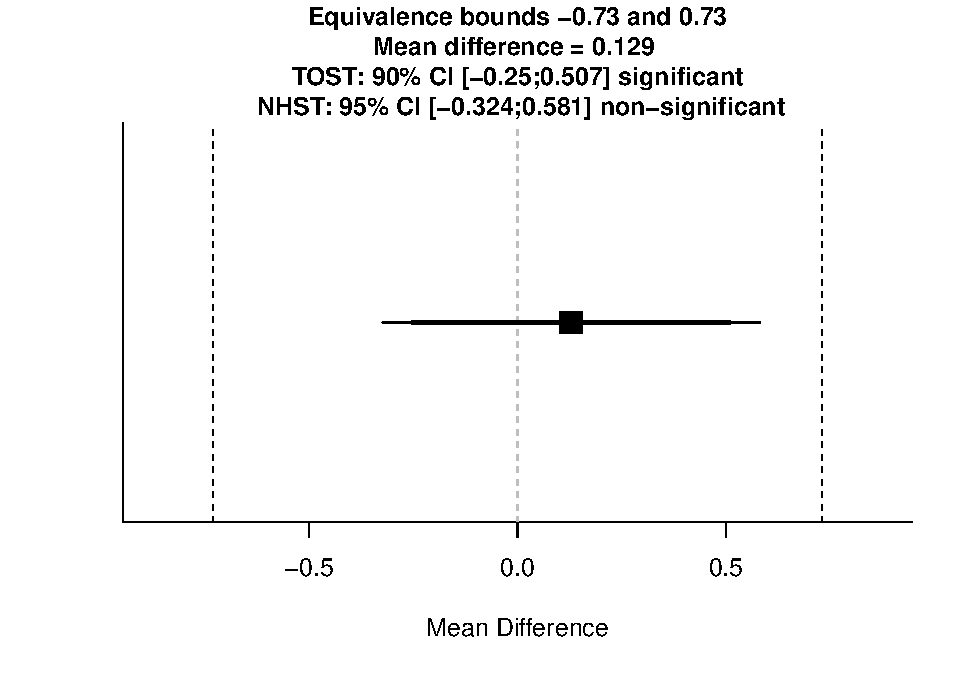
\includegraphics{manuscript_files/figure-latex/unnamed-chunk-5-1.pdf}
\caption{}
\end{figure}

\begin{verbatim}
## Using alpha = 0.05 the meta-analysis was significant, Z = 20, p = 2.753624e-89
## Using alpha = 0.05 the equivalence test was significant, Z = -13.33333, p = 7.406413e-41TOST results:
##   Z-value 1 p-value 1 Z-value 2    p-value 2
## 1  53.33333         0 -13.33333 7.406413e-41
## 
## Equivalence bounds (Cohen's d):
##   low bound d high bound d
## 1        -0.1          0.1
## 
## TOST confidence interval:
##   Lower Limit 90% CI Upper Limit 90% CI
## 1         0.05506544         0.06493456
\end{verbatim}

We see that indeed, all effect size estimates are measured with such
high precision, we can conclude that they fall within the equivalence
bound of d = -0.1 and d = 0.1. However, note that all of the effects are
also statistically significant - so, the the effects are statistically
different from zero, and practically equivalent.

\emph{Hyde, J. S., Lindberg, S. M., Linn, M. C., Ellis, A. B., \&
Williams, C. C. (2008). Gender similarities characterize math
performance. Science, 321(5888), 494-495.}

~

~

\section{Independent Groups Equivalence
Test}\label{independent-groups-equivalence-test}

~

\subsection{Independent Groups Student's Equivalence
Test}\label{independent-groups-students-equivalence-test}

Eskine (2013) showed that participants who had been exposed to organic
food were substantially harsher in their moral judgments relative to
those exposed to control (d = 0.81, 95\% CI: {[}0.19, 1.45{]}). A
replication by Moery \& Calin-Jageman (2016, Study 2) did not observe a
significant effect (Control: n = 95, M = 5.25, SD = 0.95, Organic Food:
n = 89, M = 5.22, SD = 0.83). Following Simonsohn's (2015)
recommendation the equivalence bound was set to the effect size the
original study had 33\% power to detect (with n = 21 in each condition,
this means the equivalence bound is d = 0.48, which equals a difference
of 0.384 on a 7-point scale given the sample sizes and a pooled standard
deviation of 0.894). Using a TOST equivalence test with alpha = 0.05,
assuming equal variances, and equivalence bounds of d = -0.43 and d =
0.43 is significant, t(182) = -2.69, p = 0.004. We can reject effects
larger than d = 0.43.

\begin{figure}[htbp]
\centering
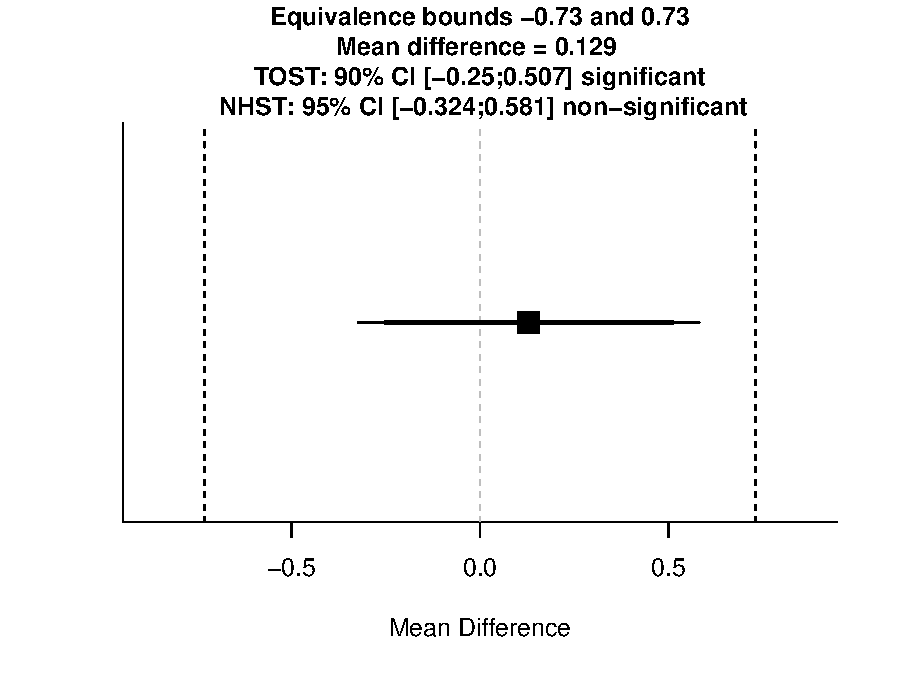
\includegraphics{manuscript_files/figure-latex/unnamed-chunk-6-1.pdf}
\caption{}
\end{figure}

\begin{verbatim}
## Using alpha = 0.05 Student's t-test was non-significant, t(182) = 0.2274761, p = 0.8203089
## Using alpha = 0.05 the equivalence test based on Student's t-test was significant, t(182) = -2.684218, p = 0.003970479TOST results:
##   t-value 1    p-value 1 t-value 2   p-value 2  df
## 1   3.13917 0.0009885653 -2.684218 0.003970479 182
## 
## Equivalence bounds (raw scores):
##   low bound raw high bound raw
## 1        -0.384          0.384
## 
## TOST confidence interval:
##   Lower Limit 90% CI raw Upper Limit 90% CI raw
## 1             -0.1880364              0.2480364
\end{verbatim}

\emph{Moery, E., \& Calin-Jageman, R. J. (2016). Direct and Conceptual
Replications of Eskine (2013): Organic Food Exposure Has Little to No
Effect on Moral Judgments and Prosocial Behavior. Social Psychological
and Personality Science, 7(4), 312-319.
\url{https://doi.org/10.1177/1948550616639649} }

~

\subsection{Independent Groups Welch's Equivalence
Test}\label{independent-groups-welchs-equivalence-test}

Deary, Thorpe, Wilson, Starr, and Whally (2003) report the IQ scores of
79,376 children in Scotland (39,343 girls and 40,033 boys). The IQ score
for girls (M = 100.64, SD = 14.1) girls and boys (100.48, SD = 14.9) was
non-significant. With such a huge sample, we can examine whether the
data is equivalent using very small equivalence bounds, such as -0.05
and 0.05. Because sample sizes are unequal, and variances are unequal,
Welch's t-test is used, and we can conclude IQ scores are indeed
equivalent, based on equivalence bounds of -0.05 and 0.05.

\begin{figure}[htbp]
\centering
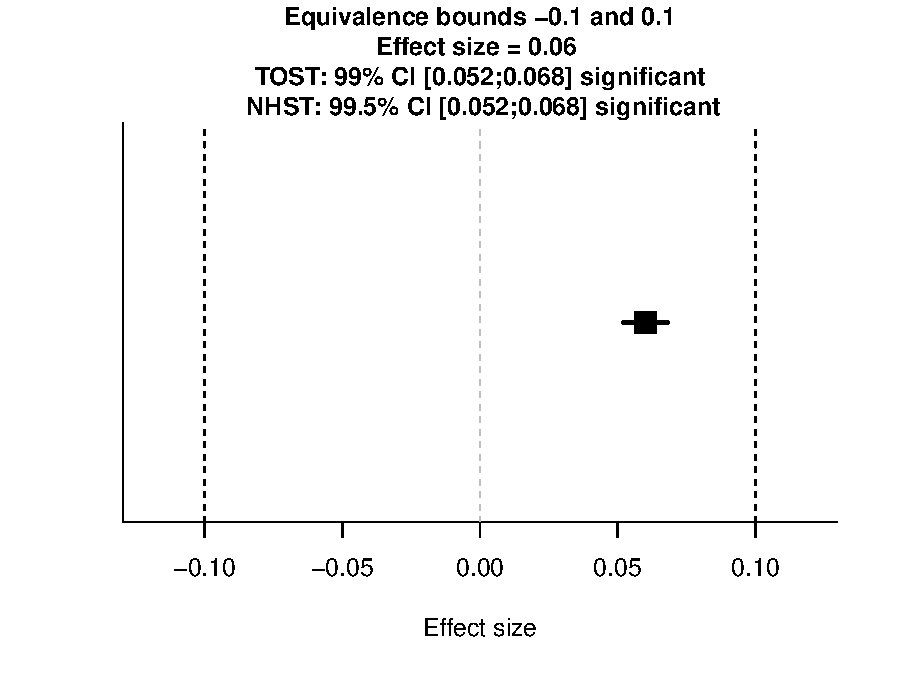
\includegraphics{manuscript_files/figure-latex/unnamed-chunk-7-1.pdf}
\caption{}
\end{figure}

\begin{verbatim}
## Using alpha = 0.05 Welch's t-test was non-significant, t(79260.94) = 1.554136, p = 0.1201559
## Using alpha = 0.05 the equivalence test based on Welch's t-test  was significant, t(79260.94) = -5.490723, p = 2.007585e-08TOST results:
##   t-value 1    p-value 1 t-value 2    p-value 2       df
## 1  8.598995 4.092652e-18 -5.490723 2.007585e-08 79260.94
## 
## Equivalence bounds (Cohen's d):
##   low bound d high bound d
## 1       -0.05         0.05
## 
## Equivalence bounds (raw scores):
##   low bound raw high bound raw
## 1    -0.7252758      0.7252758
## 
## TOST confidence interval:
##   Lower Limit 90% CI raw Upper Limit 90% CI raw
## 1           -0.009341433              0.3293414
\end{verbatim}

\emph{Deary, I. J., Thorpe, G., Wilson, V., Starr, J. M., \& Whalley, L.
J. (2003). Population sex differences in IQ at age 11: The Scottish
mental survey 1932. Intelligence, 31(6), 533-542.}

~

~

\section{One-Sample Equivalence Test}\label{one-sample-equivalence-test}

~

Lakens, Semin, \& Foroni (2012) examined whether the color of Chinese
ideographs (white vs.~black) would bias whether participants judged that
the ideograph correctly translated positive, neutral, or negative words.
In Study 4 the prediction was that participants would judge negative
words to be correctly translated by black ideographs above guessing
average, but no effects were predicted for translations in the other 5
between subject conditions in the 2 (ideograph color: white vs.~black) x
3 (word meaning: positive, neutral, negative) design. The table below is
a summary of the data in all 6 conditions:

\begin{longtable}[]{@{}lllllllll@{}}
\toprule
Color & Valence & M & \% & SD & t & df & p & d\tabularnewline
\midrule
\endhead
White & Positive & 6.05 & 50.42 & 1.50 & 0.15 & 20 & .89 &
.03\tabularnewline
White & Negative & 6.68 & 55.67 & 1.70 & 1.75 & 18 & .10 &
.40\tabularnewline
White & Neutral & 5.95 & 49.58 & 1.40 & 0.87 & 19 & .87 &
.04\tabularnewline
Black & Positive & 6.45 & 53.75 & 1.91 & 1.06 & 19 & .30 &
.24\tabularnewline
Black & Negative & 6.95 & 57.92 & 1.15 & 3.71 & 19 & .00 &
.80\tabularnewline
Black & Neutral & 5.71 & 47.58 & 1.79 & 0.73 & 20 & .47 &
.16\tabularnewline
\bottomrule
\end{longtable}

With 19 to 21 participants in each between subject condition, the study
had 80\% power to detect equivalence with equivalence bounds of -0.68 to
d = 0.68.

\begin{verbatim}
## The required sample size to achieve 80 % power with equivalence bounds of -0.68 and 0.68 is 19
\end{verbatim}

\begin{verbatim}
## [1] 18.52043
\end{verbatim}

When we perform 5 equivalence tests using equivalence bounds of -0.68
and 0.68, using a Holm-Bonferroni sequential procedure to control error
rates, we can conclude statistical equivalence for the data in row 1, 3,
and 6, but the conclusion is undetermined for tests 2 and 4, where the
data is neither significantly different from guessing average, nor
statistically equivalent. For example, performing the test for the data
in row 6:

\begin{figure}[htbp]
\centering
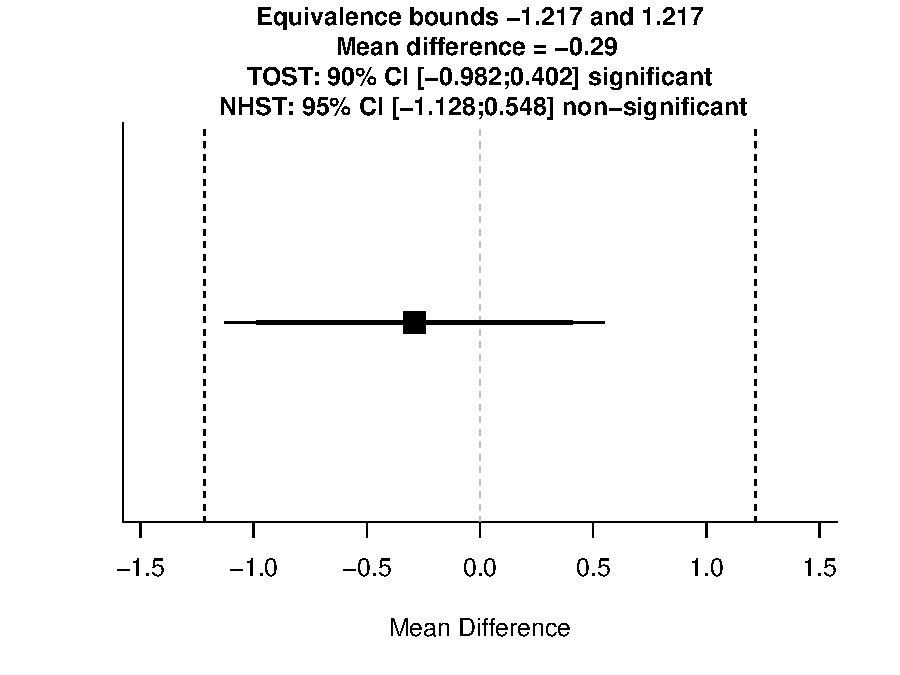
\includegraphics{manuscript_files/figure-latex/unnamed-chunk-9-1.pdf}
\caption{}
\end{figure}

\begin{verbatim}
## Using alpha = 0.05 the NHST one-sample t-test was non-significant, t(19) = -0.724536, p = 0.4775649
## Using alpha = 0.05 the equivalence test was significant, t(19) = 2.316516, p = 0.01592727TOST results:
##   t-value 1  p-value 1 t-value 2    p-value 2 df
## 1  2.316516 0.01592727 -3.765588 0.0006543016 19
## 
## Equivalence bounds (Cohen's d):
##   low bound d high bound d
## 1       -0.68         0.68
## 
## Equivalence bounds (raw scores):
##   low bound raw high bound raw
## 1       -1.2172         1.2172
## 
## TOST confidence interval:
##   Lower Limit 90% CI raw Upper Limit 90% CI raw
## 1             -0.9820961              0.4020961
\end{verbatim}

It is clear I should have been more tentative in my conclusions in this
study. Not only can I not conclude equivalence in some of the
conditions, the equivalence bound I had 80\% power to detect is very
large, meaning the possibility that there are theoretically interesting
but smaller effects remains.

\emph{Lakens, D., Semin, G. R., \& Foroni, F. (2012). But for the bad,
there would not be good: Grounding valence in brightness through shared
relational structures. Journal of Experimental Psychology: General,
141(3), 584-594. \url{https://doi.org/10.1037/a0026468} }

~

~

\section{Equivalence test for
correlations}\label{equivalence-test-for-correlations}

~

Olson, Fazio, and Hermann (2007) reported correlations between implicit
and explicit measures of self-esteem, such as the IAT, Rosenberg's
self-esteem scale, a feeling thermometer, and trait ratings. In Study 1
71 participants completed the self-esteem measures. Because no
equivalence bounds are mentioned, we can see which equivalence bounds
the researchers would have 80\% power to detect.

\begin{verbatim}
## The required sample size to achieve 80 % power with equivalence bounds of -0.24 and 0.24 is 71 pairs
\end{verbatim}

\begin{verbatim}
## [1] 70.05703
\end{verbatim}

With 71 pairs of observations between measures, the researchers have
80\% power for equivalence bounds of r = -0.24 and r = 0.24.

The correlations observed by Olson et al (2007), Study 1, are presented
in the table below (significant correlations are flagged by an
asteriks).

\begin{longtable}[]{@{}lllll@{}}
\toprule
Measure & IAT & Rosenberg & Feeling thermometer & Trait
ratings\tabularnewline
\midrule
\endhead
IAT & - & -.12 & -.09 & -.06\tabularnewline
Rosenberg & & - & .62* & .09\tabularnewline
Feeling thermometer & & & - & .29*\tabularnewline
Trait ratings & & & & -\tabularnewline
\bottomrule
\end{longtable}

We can test each correlation, for example the correlation between the
IAT and the Rosenberg self-esteem scale of -0.12, given 71 participants,
and using equivalence bounds of r\_U = 0.24 and r\_L = -0.24.

\begin{figure}[htbp]
\centering
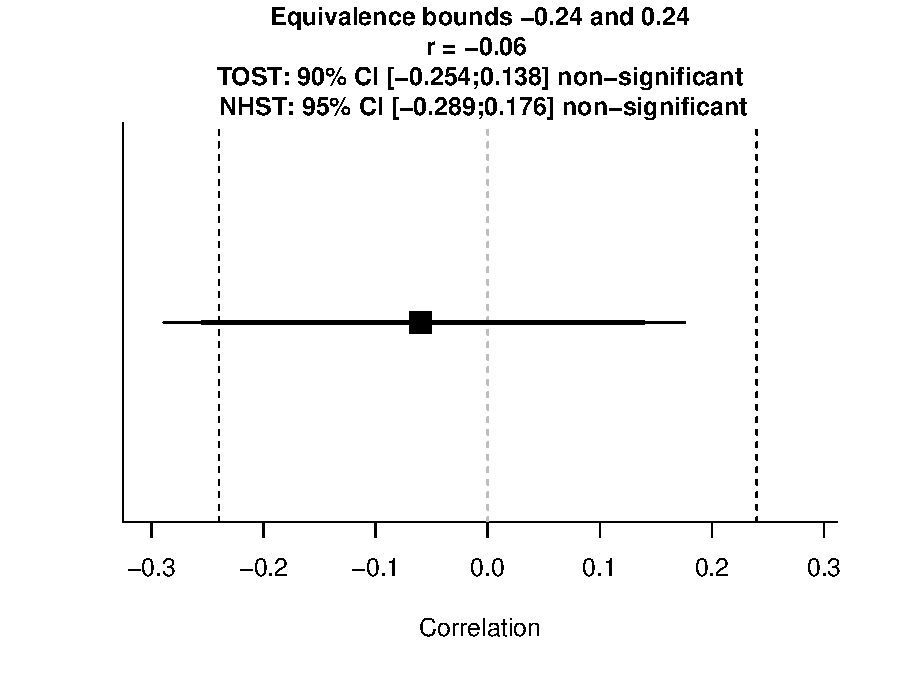
\includegraphics{manuscript_files/figure-latex/unnamed-chunk-11-1.pdf}
\caption{}
\end{figure}

\begin{verbatim}
## Using alpha = 0.05 the NHST t-test was non-significant, p = 0.6191585
## Using alpha = 0.05 the equivalence test was non-significant, p = 0.06386793TOST results:
##     p-value 1  p-value 2
## 1 0.005971455 0.06386793
## 
## Equivalence bounds (r):
##   low bound r high bound r
## 1       -0.24         0.24
## 
## TOST confidence interval:
##   Lower Limit 90% CI raw Upper Limit 90% CI raw
## 1             -0.2538652              0.1384997
\end{verbatim}

We see that none of the correlations can be declared to be statistically
equivalent. Instead, the tests yield undetermined outcomes: the
correlations are not significantly different from 0, nor statistically
equivalent.

\emph{Olson, M. A., Fazio, R. H., \& Hermann, A. D. (2007). Reporting
tendencies underlie discrepancies between implicit and explicit measures
of self-esteem. Psychological Science, 18(4), 287-291.}

\section{Discussion}\label{discussion}

\newpage

\section{References}\label{references}

Button, K. S., Kounali, D., Thomas, L., Wiles, N. J., Peters, T. J.,
Welton, N. J., . Lewis, G. (2015). Minimal clinically important
difference on the Beck Depression Inventory - II according to the
patient's perspective. Psychological Medicine, 45(15), 3269-3279.
\url{https://doi.org/10.1017/S0033291715001270}

Burriss, R. P., Troscianko, J., Lovell, P. G., Fulford, A. J. C.,
Stevens, M., Quigley, R., . Rowland, H. M. (2015). Changes in Women's
Facial Skin Color over the Ovulatory Cycle are Not Detectable by the
Human Visual System. PLOS ONE, 10(7), e0130093.
\url{https://doi.org/10.1371/journal.pone.0130093}

\setlength{\parindent}{-0.5in} \setlength{\leftskip}{0.5in}

\hypertarget{refs}{}
\hypertarget{ref-lakens_equivalence_2017}{}
Lakens, D. (2017). Equivalence Tests: A Practical Primer for t Tests,
Correlations, and Meta-Analyses. \emph{Social Psychological and
Personality Science}, \emph{8}(4), 355--362.
doi:\href{https://doi.org/10.1177/1948550617697177}{10.1177/1948550617697177}






\end{document}
